\section{Data}

\subsection{Light Bulbs and the Solar spectrum}
For this part, we plotted the meassured intensity of the light as a function of 
wavelengths, and determined at which index of wavelength, the peak of highest
intensity was at. This wavelength corresponds to a temperature as described in
\cref{eq:wien} to calculate the temperature $T$.
For the three meassurements of the solar spectrum, we took an average. All the
temperatures are shown in \cref{tab:temp}.
\begin{table}[h]
\centering
\begin{tabular}[h]{lr}
\toprule
Source & Temperature\\
\midrule
Halogen       & $\SI{4736}{\kelvin}$\\
Diode         & $\SI{4842}{\kelvin}$\\
Energy-saving & $\SI{4829}{\kelvin}$\\
Solar average & $\SI{5663}{\kelvin}$\\
\bottomrule
\end{tabular}
\caption{Surface temperatures of the given sources, as determined by wiens
displacement law.}
\label{tab:temp}
\end{table}
Our meassurements of the three lamps are shown compared to the three solar
spectra on \cref{diode}, \cref{halogen} and \cref{Energy-saving}.

\begin{figure}[h!]
\centering
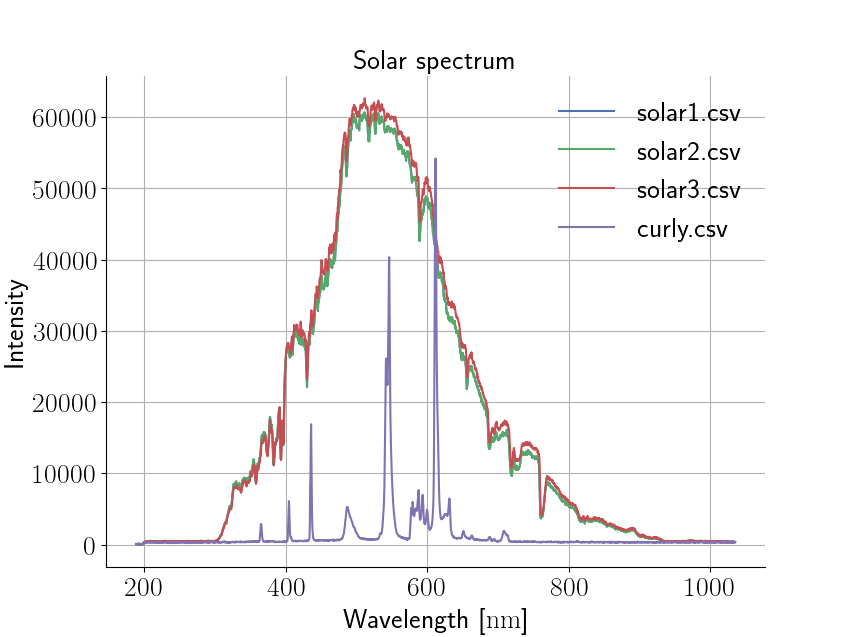
\includegraphics[width=0.65\textwidth]{SolarComparison0}
\caption{The spectrum of the diode-based lamp compared to the three meassured spectra of
the sun.} 
\label{diode}
\end{figure}

\begin{figure}[h!]
\centering
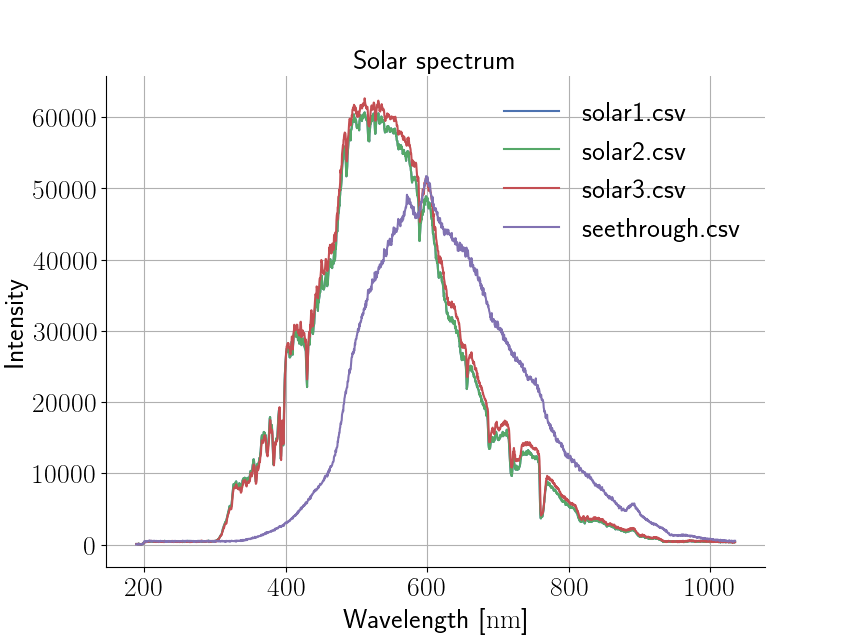
\includegraphics[width=0.65\textwidth]{SolarComparison1}
\caption{Halogen}
\label{halogen}
\end{figure}

\begin{figure}[h!]
\centering
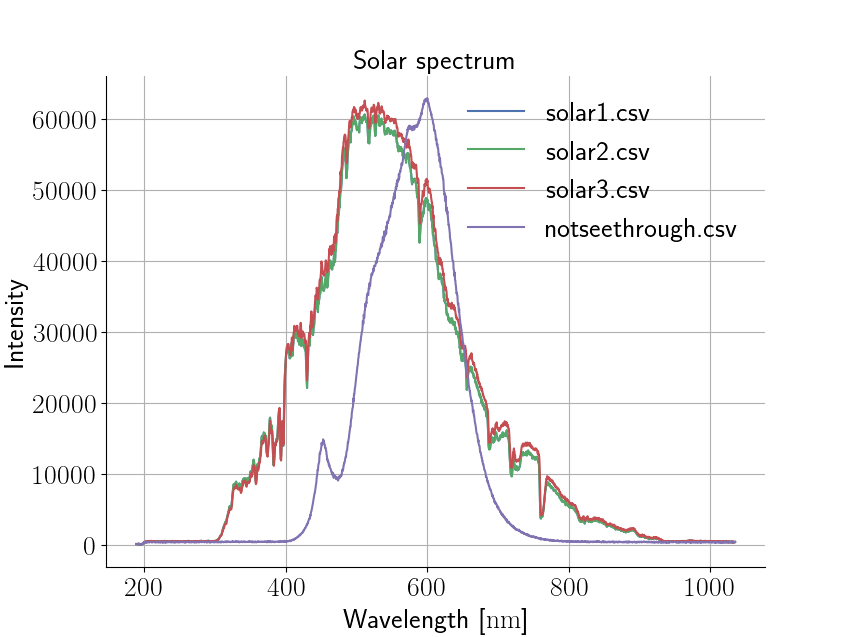
\includegraphics[width=0.65\textwidth]{SolarComparison2}
\caption{Energy-saving lamp}
\label{Energy-saving}
\end{figure}

\subsubsection{Comparison}
The question is, which of our three lamps best represtent the solar spectrum.
From the three figures \cref{diode}, \cref{halogen} and \cref{Energy-saving},
it can be seen, that:

\paragraph{diode}
This spectrum is discrete. Some of the wavelengths are similar to that of the
solar, but it is certainly not a blackbody.

\paragraph{halogen}
This spectrum has its peak displaced further into the yellow color, whereas the
sun has a greenish peak. Nonetheless, it is certainly a better approximation
than that of the diode.

\paragraph{energy-saving}
This spectrum has its peak nearest that of the solar spectrum, and thus shares
the same color. Though it has a smaller full-width-half-maxima than that of the
halogen lamp.

\subsection{Fraunhofer lines}
\begin{figure}[h]
\centering
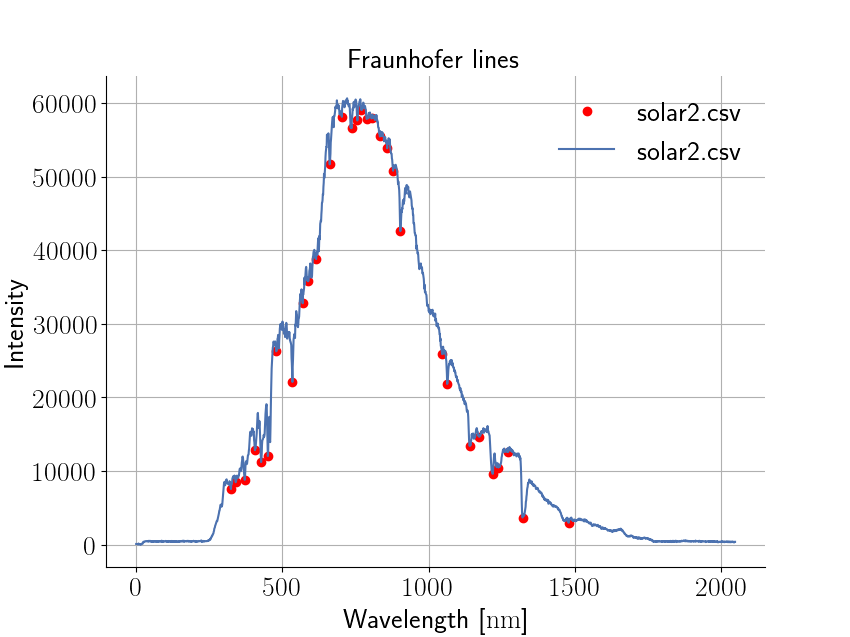
\includegraphics[width=0.65\textwidth]{Fraunhofer}
\caption{The Solar spectra with the local extrema points used for
classification of the Fraunhofer lines}
\label{frauenhofer}
\end{figure}

Comparing the found extremas with the Fraunhofer lines, we have meassured the
following

\subsection{Emission spectrum of element lamps}

In this part of the experiment we look at the energy transitions of different elements by looking at the spectre of lamps filled with the elements on gasform, which is excited by a voltage running over the lamp causing the element to emit light. We've made a spectrum for Xenon, mercury, helium, neon and argon. We will go into depth with the 3 first spectres, finding the energy transistions and lower and upper  electron configurations for the transitions.The energy transitions are primarily governed by the the main quantum number $n$ and the fine structure of atoms which arises due to relativistic corrections of the electrons mass and the coupling of the electrons orbital angular momentum and the electrons spin.\\
 When describing the electron configurations of atoms one will usually use the spectroscopic notation where the atom has certain energy shells and subshells, where the shells a determined by the primary quantum number and the subshells differs by the orbital angular momentum $l$. The energy differences in the subshells are a consequence of the finestructure. The superscript after $l$ indicates the number of electrons in a given subshell. Each shell can hold $2n^2$ electrons with $2(2l+1)$ electrons in each subshell. Some of the possible configurations will not be allowed due to Pauli's exclusion principle. Besides from the subshells the will be even finer splittings in the energy levels due to the coupling of the nucleus and the total angular momentum of the electrons (L+S=J). 
 
 %husk at ændre her og gøre mindre 

\tabcolsep=0.11cm
\begin{tabular}{|l|l|l|l|l|l|}\hline
	Xe & \multicolumn{5}{c}{}  \\ 
	&  obs. wavelength (nm) & det. wavelength (nm) & Lower level (conf., J) & Upper level (conf., J) & Energy shift \\
	&  \multirow{2}{*}{462} & 461.18882 & 5p5(2P3/2)6s  2 & 5p5(2P3/2)7p  1 	& 67 067.547 	- 	88 744.559   \\
	& &  462.42756 & 5p56s 	 2 & 5p57p  2 &67 067.547 	- 	88 686.500 \\
	&  467 & 467.12258 & $5p^5 6s$  2 & $5p^5 7p$   3 &  67 067.547 	- 	88 469.213 \\
	&  472 & 473.41518 &  $5p^5 6s$  1 & $5p^5 6p$  2 & 68 045.156 	- 	89 162.356 \\
	&  823 & 823.16336 & $5p^5 6s$  2 & $5p^5 6p$  2 & 67 067.547 	- 	79 212.465 \\
	&  828 & 828.01162 &  $5p^5 6s$  1 & $5p^5 6p$  0 & 68 045.156 	- 	80 118.962 \\
	&  882 & 881.94106 &  $5p^5 6s$  2 & $5p^5 6p$  3 & 67 067.547 	- 	78 403.061 \\
	&  894 & 893.0830 & $5p^5 6s$  1 & $5p^5 6p$  1 & 77 185.041 	- 	88 379.126 	\\
	&  895 & 895.22509 & $5p^5 6s$  1 & $5p^5 6p$  2 & 68 045.156 	- 	79 212.465\\
	&  904 & 904.54466 & $5p^5 6s$ 	 2 & $5p^5 6p$  2 & 67 067.547 	- 	78 119.798 \\
	&  916 & 916.26520  &  $5p^5 6s$  1 &  $5p^5 6p$  1 & 68 045.156 	- 	78 956.031 \\ 
	 \hline
	         %% here
\end{tabular}

\tabcolsep=0.11cm
\begin{tabular}{|l|l|l|l|l|l|}\hline
	Hg & \multicolumn{5}{c}{} \\ 
	&  obs. wavelength (nm) & det. wavelength (nm) & Lower level (conf., J) & Upper level (conf., J) & Energy shift \\
	& \multirow{2}{*}{313} & 313.15547 & 5d106s6p  1& 5d106s6d 1& 39 412.237  	- 	71 336.005\\
	& & 313.18443 & 5d106s6p  1& 5d106s6d  2& 39 412.237  	- 	71 333.053\\
	& 364 & 365.01580 & 5d106s6p  2 &  5d106s6d  3 & 44 042.909  	- 	71 431.180 \\
	& 405 & 404.65650 & 5d106s6p  0 & 5d106s7s  1& 37 644.982  	- 	62 350.325\\
	& 435 & 435.83350 & 5d106s6p  1& 5d106s7s  1& 39 412.237  	- 	62 350.325 \\
	& 545 & 546.07500 & 5d106s6p  2& 5d106s7s  1& 44 042.909  	- 	62 350.325\\
	& 578 & 576.96100 & 5d106s6p  1& 5d106s6d  2& 54 068.6829 	- 	71 396.073\\
	& 750 & \multicolumn{4}{c}{no data}\\
	\hline
\end{tabular}

\tabcolsep=0.11cm
\begin{tabular}{|l|l|l|l|l|l|}\hline
	He & \multicolumn{5}{c}{} \\ 
	&  obs. wavelength (nm) & det. wavelength (nm) & Lower level (conf., J) & Upper level (conf., J) & Energy shift \\
	& \multirow{2}{*}{318} & 318.7744390& 1s2s  1& 1s4p  1& [159 855.9743297] 	- 	[191 217.049963] \\
	& & 318.7745305 & 1s2s  1& 1s4p  2& [159 855.9743297] 	- 	[191 217.040967] \\
	& \multirow{5}{*}{358}& 358.7270 & 1s2p  2& 1s9d  1& [169 086.7664725] 	- 	[196 955.22825838] \\
	& & 358.7270 & 1s2p  2& 1s9d  2& [169 086.7664725] 	- 	[196 955.22664143]\\
	& & 358.7270 & 1s2p  2& 1s9d  3& [169 086.7664725] 	- 	[196 955.22652671]\\'
	& & 358.7270 & 1s2p  1& 1s9d  1& [169 086.8428979] 	- 	[196 955.22825838]\\
	& & 358.7270 & 1s2p  1& 1s9d  2& [169 086.8428979] 	- 	[196 955.22664143]\\
	& 395 & 396.47291& 1s2s  0& 1s4p  1& [166 277.440141]  	- 	[191 492.711909] \\
	& \multirow{5}{*}{402} & 402.61914 &1s2p  2& 1s5d 1& [169 086.7664725] 	- 	[193 917.16138710]\\
	& & 402.61914& 1s2p  2&1s5d  2& [169 086.7664725] 	- 	[193 917.15192855] \\'
	& & 402.61914& 1s2p  2&1s5d  3& [169 086.7664725] 	- 	[193 917.15128741] \\
	& & 402.61914& 1s2p  1&1s5d  1& [169 086.8428979] 	- 	[193 917.16138710]  \\
	& & 402.61914& 1s2p  1&1s5d  2&[169 086.8428979] 	- 	[193 917.15192855] \\
	& 438& 438.79296 & 1s2p  1&  1s5d  2& [171 134.896946]  	- 	[193 918.28990114]\\'
	& \multirow{5}{*}{447}& 447.14802& 1s2p  2& 1s4d  1& [169 086.7664725] 	- 	[191 444.5006512]\\
	& & 447.14802 & 1s2p  2& 1s4d  2& [169 086.7664725] 	- 	[191 444.4821307]\\
	& & 447.14802 & 1s2p  2& 1s4d  3& [169 086.7664725] 	- 	[191 444.4809292]\\
	& & 447.14802 & 1s2p  1& 1s4d  1& [169 086.8428979] 	- 	[191 444.5006512] \\
	& & 447.14802 & 1s2p  1& 1s4d  2& [169 086.8428979] 	- 	[191 444.4821307]\\
	& \multirow{2}{*}{472}& 471.31457& 1s2p  2& 1s4s 1& [169 086.7664725] 	- 	[190 298.113260] \\
	& & 471.31457&  1s2p  1&  1s4s  1& [169 086.8428979] 	- 	[190 298.113260] \\
	& 491 & 492.19313 & 1s2p  1&  1s4d  2& [171 134.896946]  	- 	[191 446.4557405]\\
	&502 & 501.56783& 1s2s  0& 1s3p  1& [166 277.440141]  	- 	[186 209.364940] \\
	\hline
	
\end{tabular}

The tabels has been filled out using the database . By determining the wavelength of the most visible peaks in our spectre, we've compared it to the transitions shown on the NIST website and then chosen the wavelength with highest relative intensity to take the data from. In the case of multiple transistions having same relative intensity and wavelength, they have all been noted. For each observed wavelength we've noted the wavelength that we think we've observed, the upper and lower level electronic configurations and total angular momentum, and the energy shift. 




\subsection{Absorption Spectroscopy}
\begin{figure}[h]
\centering
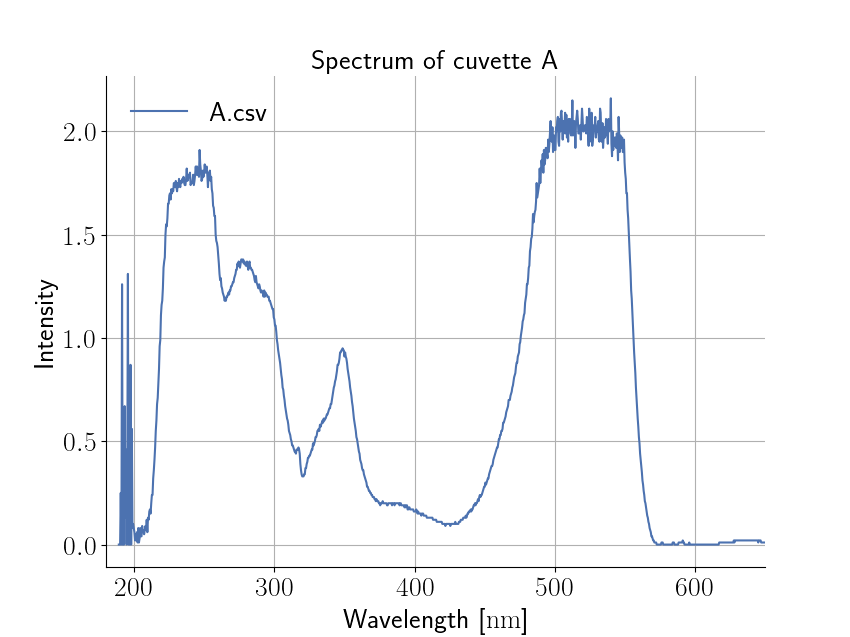
\includegraphics[width=0.65\textwidth]{absA}
\caption{Spectrum of cuvette A: This might just be Rhodamine 6G}
\label{fig:absA}
\end{figure}
\begin{figure}[h]
\centering
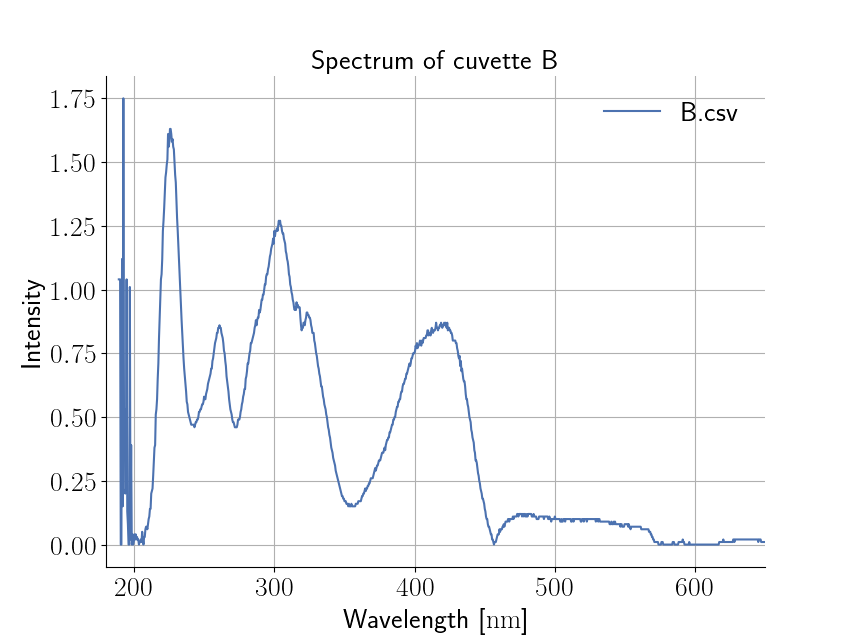
\includegraphics[width=0.65\textwidth]{absB}
\caption{Spectrum of cuvette B. As this seems different from all spectra of
figure 13 (in lab guide), this might just be Kaliumhexacyanoferrat (III)}
\label{fig:absB}
\end{figure}
\begin{figure}[h]
\centering
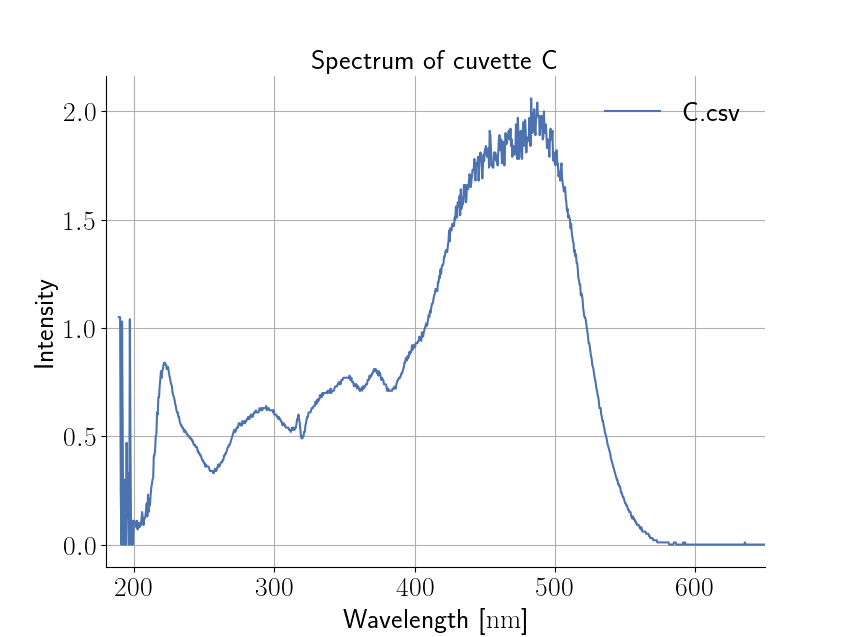
\includegraphics[width=0.65\textwidth]{absC}
\caption{Spectrum of cuvette C. This might just be DCM}
\label{fig:absC}
\end{figure}
